\documentclass[11pt,a4paper]{article}

\usepackage[utf8]{inputenc}
\usepackage[T1]{fontenc}
\usepackage{lmodern}
\usepackage[english]{babel}
\usepackage[margin=1in]{geometry}
\usepackage{microtype}
\usepackage{parskip}
\usepackage{graphicx}
\usepackage{booktabs}
\usepackage{array}
\usepackage{enumitem}
\usepackage{caption}
\usepackage{float}
\usepackage{xcolor}
\usepackage{tikz}
\usetikzlibrary{arrows.meta, positioning, shapes.geometric, shapes.misc}
\usepackage{hyperref}
\hypersetup{
    colorlinks=true,
    linkcolor=blue!50!black,
    citecolor=blue!50!black,
    urlcolor=blue!50!black,
    pdftitle={A Manager's Guide to the Project Management Triangle},
    pdfauthor={Norbert Nopper}
}

\graphicspath{{figures/}}

\title{A Manager's Guide to the Project Management Triangle}
\author{Norbert Nopper}
\date{\today}

\begin{document}
\maketitle

\begin{abstract}
\noindent
The \emph{Project Management Triangle} --- relating scope, time, and cost as
interdependent constraints --- is a well-established model in the project
management literature (Barnes, 1969; Kerzner, 2017; Project Management
Institute, 2017). Several extensions and adjacent contributions exist:
quality as the implicit outcome of constraint balance (Atkinson, 1999),
time-boxed iteration fixing time and cost while varying scope (Beck, 1999;
Sutherland \& Schwaber, 2020), deferred commitment in Lean development
(Poppendieck \& Poppendieck, 2003), buffer management in the Theory of
Constraints (Goldratt, 1997), and strategic pivoting in Lean Startup
methodology (Ries, 2011).

The individual ingredients of this document are therefore not new. What
this document offers is a \textbf{novel synthesis}: a single, explicit
framework that unifies these scattered ideas into a small, named set of
configurations and a structured rule for moving between them. Concretely:

\begin{enumerate}[leftmargin=*]
  \item \textbf{A unified Fixed/Variable configuration map.} Each of the
  three constraints is classified as either \emph{Fixed} (F) or
  \emph{Variable} (V) at any point in time. All $2^3 = 8$ binary
  assignments are enumerated, the two degenerate cases (all-fixed,
  all-variable) are identified as non-viable, and the six valid
  configurations are aligned with established delivery patterns. The
  enumeration itself is not new --- Wysocki (2014) already presents a
  ``flexibility matrix'' over the same constraints, and DSDM (Stapleton,
  2003) prioritises constraints in a comparable fashion. The contribution
  here is the \emph{shared, neutral vocabulary}: the same configurations
  under method-agnostic F/V labels rather than method-specific brand
  names, and a single map covering all six valid cases on equal footing.

  \item \textbf{Explicit, named configuration pivoting (the principal
  novel element).} Building on Ries' (2011) notion of the pivot as a
  strategic course correction, this document defines \emph{configuration
  pivoting}: the deliberate re-assignment of the F/V status of the
  triangle's constraints. Adjacent practices already do this implicitly
  --- rolling-wave planning, re-baselining (Project Management Institute,
  2017), and Scrum's empirical inspect-and-adapt cycle (Sutherland \&
  Schwaber, 2020) all adjust constraints in flight. What this document
  adds is to make the act explicit and named, with a procedural rule: the
  pivot is \textbf{anchored to the current actual values} of scope, time,
  and cost at the moment of re-configuration --- not to the original
  baseline. Naming the action and the anchor is the contribution; the
  practice itself has analogues.

  \item \textbf{Intentionality as an explicit management decision.} The
  F/V assignment is treated as a first-class, openly negotiated decision
  rather than an emergent property of execution. This is more a framing
  argument than an empirical result, but framing matters: leaving the
  assignment implicit --- as conventional triangle usage does --- is a
  recurring source of unacknowledged trade-offs and stakeholder
  misalignment.
\end{enumerate}

\medskip
\noindent\textbf{Scope and limitations.} This is a practitioner-oriented
synthesis, not a peer-reviewed empirical study. No quantitative validation
is offered. The document is intended as a manager's reference: a
vocabulary and a procedure, not a proof.
\end{abstract}

\medskip
\noindent\textbf{Keywords:} project management triangle, iron triangle,
triple constraint, scope, time, cost, quality, fixed/variable constraints,
pivoting, configuration management, agile, lean, scrum.

\tableofcontents
\bigskip

\section{How to Use This Document}
\label{sec:how-to-use}

This guide is intended as a working reference, not background reading.
Two practical habits are enough to put it to use:

\begin{itemize}[leftmargin=*]
  \item \textbf{At kickoff and at every review,} ask out loud and record
  the answer: \emph{Which of scope, time, and cost is Fixed? Which is
  Variable?} Treat the answer as a first-class artefact, alongside the
  schedule and the budget.
  \item \textbf{When something changes} --- requirements, dependencies,
  market, funding --- run a deliberate \textbf{configuration pivot}:
  capture the \emph{current actual} scope, time, and cost (not the
  original plan), then re-decide F/V from there.
  Section~\ref{sec:pivoting} describes the procedure.
\end{itemize}

If you read nothing else, read Section~\ref{sec:pivoting} (including the
worked example in Section~\ref{sec:worked-example}) and the summary table
(Section~\ref{sec:summary}).

\section{Glossary}
\label{sec:glossary}

\begin{description}[leftmargin=*]
  \item[Constraint] one of \emph{scope}, \emph{time}, \emph{cost}: the
  three coupled dimensions of the triangle.
  \item[Fixed (F)] a constraint that is locked for the current
  configuration and must be respected.
  \item[Variable (V)] the absorber: the constraint that flexes when
  reality diverges from plan.
  \item[Configuration] an assignment of F or V to each of the three
  constraints. There are $2^3 = 8$ such assignments, of which 6 are
  viable.
  \item[Quality] the implicit outcome of a configuration; not a fourth
  constraint, but the consequence of how F and V are chosen and respected
  (Atkinson, 1999).
  \item[Status quo] the \emph{current actual} values of scope, time, and
  cost at a given moment, as opposed to the original baseline.
  \item[Pivot] a deliberate, named change of configuration, anchored to
  the status quo rather than to the baseline.
\end{description}

\section{The Classic Project Management Triangle}
\label{sec:classic}

The \textbf{Project Management Triangle} (also called the \emph{Iron
Triangle} or \emph{Triple Constraint}) is a foundational model in
project management. It states that every project is constrained by three
interdependent elements:

\begin{itemize}[leftmargin=*]
  \item \textbf{Scope} --- what the project delivers (features, quality,
  requirements)
  \item \textbf{Time} --- how long the project takes (schedule, deadline)
  \item \textbf{Cost} --- how much the project spends (budget, resources)
\end{itemize}

The core insight is that these three constraints are coupled: changing
one forces a change in at least one of the others. This is often
summarised as:

\begin{quote}
\emph{``Good, fast, cheap --- pick two.''}
\end{quote}

A widely accepted extension places \textbf{Quality} at the interior of
the triangle, representing the implicit outcome that results from how
the three constraints are balanced (Atkinson, 1999; Project Management
Institute, 2017). Quality is not a fourth independent constraint --- it
is the emergent product of the trade-offs made among scope, time, and
cost. All diagrams in this document label the interior accordingly.

\begin{figure}[H]
\centering
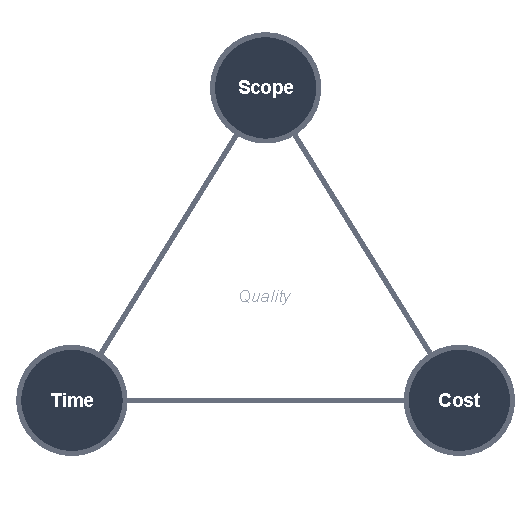
\includegraphics[width=0.42\linewidth]{classic.pdf}
\caption{Classic Project Management Triangle with quality at the
interior.}
\label{fig:classic}
\end{figure}

\section{The Dynamic Project Management Triangle}
\label{sec:dynamic}

The \textbf{Dynamic Project Management Triangle} extends the classic
model by making the fixed/variable status of each constraint an
explicit, first-class decision. At any point in a project, each of the
three elements is either:

\begin{itemize}[leftmargin=*]
  \item \textbf{Fixed (F)} --- this constraint is locked and must be
  respected.
  \item \textbf{Variable (V)} --- this constraint is the absorber; it
  flexes to accommodate changes in the other two.
\end{itemize}

The key shift is \emph{intentionality}: instead of discovering which
constraint was implicitly sacrificed after the fact, teams agree upfront
which element will absorb pressure.

\section{Pivoting in Project Management}
\label{sec:pivoting}

In traditional project management the triangle is treated as static:
constraints are agreed upon at the start and held firm. In practice,
however, projects face changing requirements, shifting priorities, and
unexpected events. \textbf{Pivoting} is the deliberate, structured act
of re-negotiating the F/V assignment in response to new information.

The concept of pivoting originates in \textbf{Lean Startup methodology}
(Ries, 2011), where a pivot means changing strategy while staying true
to the underlying mission. Applied to the Dynamic Triangle, a
configuration pivot proceeds in three steps:

\begin{enumerate}[leftmargin=*]
  \item \textbf{Take the status quo.} At the moment of the pivot, the
  current actual values of scope, time, and cost are captured as they
  stand --- not the original plan, but the real state of the project
  right now.
  \item \textbf{Re-assign fixed and variable.} From that baseline, the
  team explicitly decides which elements become fixed and which become
  variable going forward.
  \item \textbf{Continue from there.} The new configuration governs the
  project until the next deliberate pivot.
\end{enumerate}

A pivot is therefore not a reset and not an admission of failure --- it
is a structured handoff from one constraint configuration to another,
anchored to reality.

\begin{figure}[H]
\centering
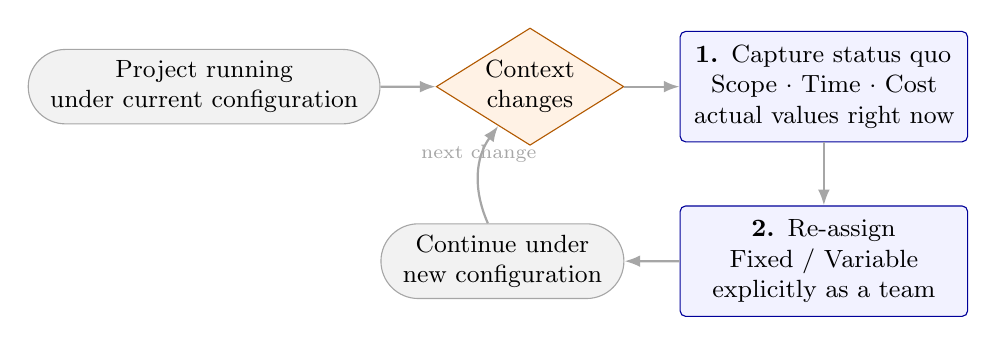
\begin{tikzpicture}[
  node distance=8mm and 7mm,
  every node/.style={font=\small},
  stateblock/.style={rounded rectangle, draw=gray!70, fill=gray!10,
                inner sep=4pt, align=center, minimum height=8mm},
  pivotstep/.style={rectangle, rounded corners=2pt, draw=blue!60!black,
               fill=blue!5, inner sep=5pt, align=center,
               minimum height=10mm, text width=33mm},
  decision/.style={diamond, draw=orange!70!black, fill=orange!10,
                   inner sep=1pt, align=center, aspect=1.6},
  arr/.style={-{Latex[length=2mm]}, thick, gray!70}
]
  \node[stateblock] (A) {Project running\\under current configuration};
  \node[decision, right=of A] (B) {Context\\changes};
  \node[pivotstep, right=of B] (C) {\textbf{1.} Capture status quo\\
                               Scope $\cdot$ Time $\cdot$ Cost\\
                               actual values right now};
  \node[pivotstep, below=of C] (D) {\textbf{2.} Re-assign Fixed / Variable\\
                               explicitly as a team};
  \node[stateblock, left=of D] (E) {Continue under\\new configuration};

  \draw[arr] (A) -- (B);
  \draw[arr] (B) -- (C);
  \draw[arr] (C) -- (D);
  \draw[arr] (D) -- (E);
  \draw[arr] (E) to[bend left=30] node[midway, above, font=\scriptsize]{next change} (B);
\end{tikzpicture}
\caption{The configuration pivot procedure.}
\label{fig:pivot}
\end{figure}

\subsection{Worked Example: Why the Anchor Matters}
\label{sec:worked-example}

The defining detail of a configuration pivot is its \emph{anchor}: the
new configuration is decided from the \textbf{current actual} state, not
from the original plan. A short example makes the difference concrete.

A team commits to a baseline: \emph{scope} of 30 features, \emph{time}
of 6 months, \emph{cost} of one 5-person team. Time and cost are fixed;
scope is the absorber (configuration V$\cdot$F$\cdot$F, the Scrum
pattern). Four months in, the actual state has diverged: 12 features are
done, a key dependency has slipped, and a hard external deadline has
appeared two months out. A pivot is triggered.

\begin{itemize}[leftmargin=*]
  \item \textbf{Baseline-anchored (the anti-pattern).} The team measures
  progress against the original 30 features and 6 months. The remaining
  18 features are treated as still owed, the original end date as still
  binding. Pressure is absorbed covertly --- overtime, quietly dropped
  quality --- because the plan on paper was never renegotiated.
  \item \textbf{Status-quo-anchored (the pivot).} The team records the
  real state right now: 12 features shipped, 2 months of runway, the
  same 5-person team. \emph{From that point}, it re-decides F/V. The new
  external deadline makes time the hard constraint; budget is opened to
  allow short-term contractors; scope for the remaining window is
  re-negotiated down to what genuinely fits. The configuration pivots to
  V$\cdot$F$\cdot$V (Ship-to-Date), explicitly and on the record.
\end{itemize}

\noindent
Both teams face the same reality. The status-quo-anchored team converts
it into an open, named decision with a sanctioned absorber; the
baseline-anchored team carries a stale plan and pays for the gap in
hidden trade-offs. The anchor, not the re-planning, is the contribution.

\section{All Configurations of Fixed and Variable Constraints}
\label{sec:configurations}

With three binary constraints there are $2^3 = \textbf{8 configurations}$.
Two of these (all-fixed and all-variable) are degenerate cases covered in
Section~\ref{sec:degenerate}. The six meaningful configurations are
enumerated below.

\subsection{Scope Fixed $\cdot$ Time Fixed $\cdot$ Cost Variable
            (Regulatory / Hard-Deadline Compliance)}

\begin{figure}[H]
\centering
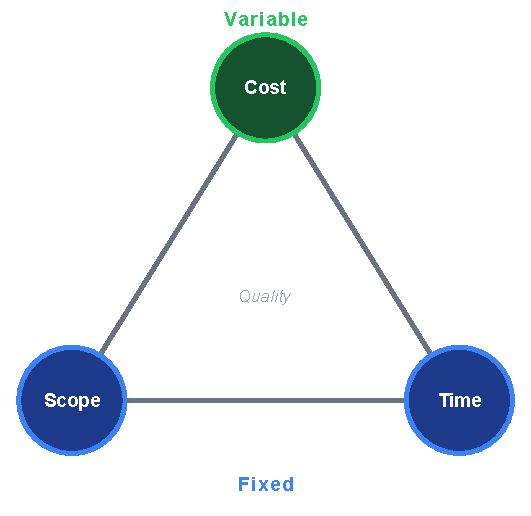
\includegraphics[width=0.40\linewidth]{perm1_FFV.pdf}
\caption{Scope Fixed, Time Fixed, Cost Variable.}
\end{figure}

\begin{center}
\begin{tabular}{ccc}
\toprule
Scope & Time & Cost \\
\midrule
F & F & \textbf{V} \\
\bottomrule
\end{tabular}
\end{center}

\noindent\textbf{What it means:} The deliverable and the deadline are
locked. Budget expands or contracts as needed.

\noindent\textbf{When to use it:} Regulatory or contractual deliverables
with hard deadlines (e.g., a compliance release that must ship before a
legal effective date). Cost overruns are acceptable; missing scope or
the deadline is not.

\noindent\textbf{Pivot signal:} Budget burn rate exceeds projections
$\to$ re-examine whether scope or time can move before escalating cost
further.

\subsection{Scope Fixed $\cdot$ Time Variable $\cdot$ Cost Fixed
            (Internal Migration / Capped-Budget Delivery)}

\begin{figure}[H]
\centering
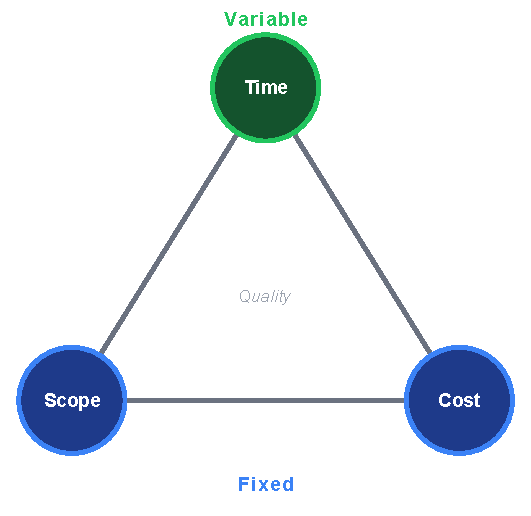
\includegraphics[width=0.40\linewidth]{perm2_FVF.pdf}
\caption{Scope Fixed, Time Variable, Cost Fixed.}
\end{figure}

\begin{center}
\begin{tabular}{ccc}
\toprule
Scope & Time & Cost \\
\midrule
F & \textbf{V} & F \\
\bottomrule
\end{tabular}
\end{center}

\noindent\textbf{What it means:} The deliverable and the budget are
locked. The schedule slips as required.

\noindent\textbf{When to use it:} Internal migrations, infrastructure
replacements, or one-shot deliverables where the output specification is
non-negotiable, the funding envelope is capped, but the launch date is
flexible (e.g., a database migration that must complete correctly within
budget but can take as long as needed). Note: this configuration is
\emph{not} a good fit for exploratory R\&D --- true R\&D usually has
variable scope (see Section~\ref{sec:perm6}).

\noindent\textbf{Pivot signal:} Repeated schedule slippage $\to$ consider
whether some scope items can be deferred to bring the timeline back
under control.

\subsection{Scope Variable $\cdot$ Time Fixed $\cdot$ Cost Fixed
            (Scrum / Agile Sprint)}

\begin{figure}[H]
\centering
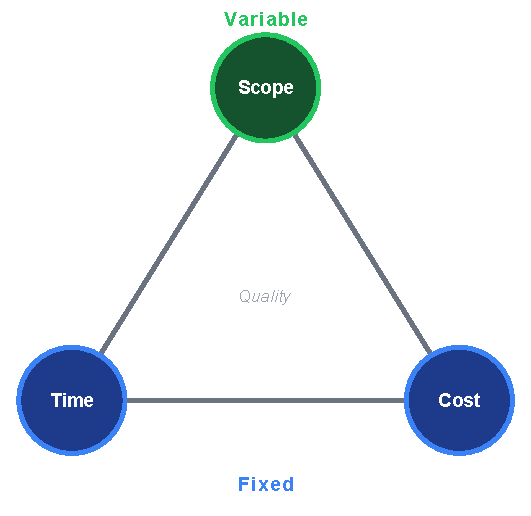
\includegraphics[width=0.40\linewidth]{perm3_VFF.pdf}
\caption{Scope Variable, Time Fixed, Cost Fixed.}
\end{figure}

\begin{center}
\begin{tabular}{ccc}
\toprule
Scope & Time & Cost \\
\midrule
\textbf{V} & F & F \\
\bottomrule
\end{tabular}
\end{center}

\noindent\textbf{What it means:} The deadline and the budget are locked.
Scope is cut or grown to fit.

\noindent\textbf{When to use it:} Time-boxed releases (e.g., a product
launch tied to a trade show) where the date and team capacity are
non-negotiable but the feature set can flex. This is the default mode of
\textbf{Scrum} --- the sprint is the fixed time-box; what ships in that
sprint is variable.

\noindent\textbf{Pivot signal:} Scope keeps growing (scope creep) $\to$
prioritise ruthlessly or reset the scope baseline before cost or time
are affected.

\subsection{Scope Fixed $\cdot$ Time Variable $\cdot$ Cost Variable
            (Cost-Plus Contract)}

\begin{figure}[H]
\centering
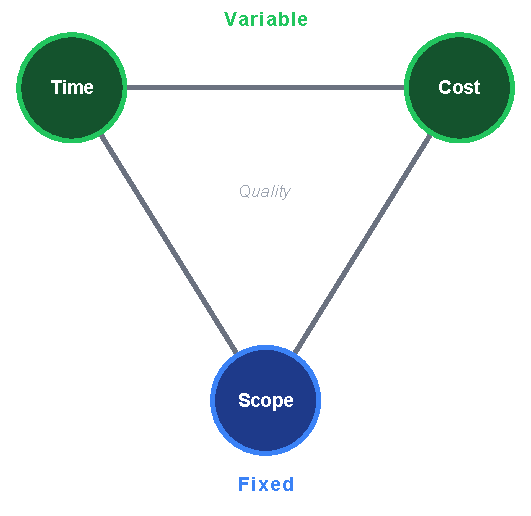
\includegraphics[width=0.40\linewidth]{perm4_FVV.pdf}
\caption{Scope Fixed, Time Variable, Cost Variable.}
\end{figure}

\begin{center}
\begin{tabular}{ccc}
\toprule
Scope & Time & Cost \\
\midrule
F & \textbf{V} & \textbf{V} \\
\bottomrule
\end{tabular}
\end{center}

\noindent\textbf{What it means:} The deliverable specification is the
only non-negotiable. Both schedule and budget flex.

\noindent\textbf{When to use it:} Safety-critical or mission-critical
systems (aerospace, medical devices) where correctness and completeness
of scope cannot be compromised under any circumstance. Common in
cost-plus government contracts.

\noindent\textbf{Pivot signal:} Both time and cost grow without bound
$\to$ the scope definition itself may be ambiguous or gold-plating is
occurring; return to scope baseline.

\subsection{Scope Variable $\cdot$ Time Fixed $\cdot$ Cost Variable
            (Ship-to-Date / Market Launch)}

\begin{figure}[H]
\centering
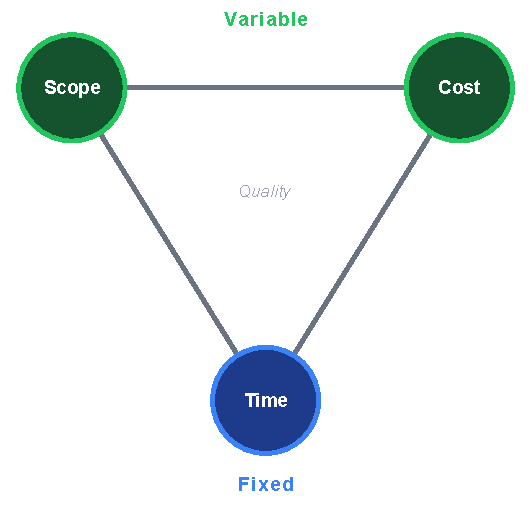
\includegraphics[width=0.40\linewidth]{perm5_VFV.pdf}
\caption{Scope Variable, Time Fixed, Cost Variable.}
\end{figure}

\begin{center}
\begin{tabular}{ccc}
\toprule
Scope & Time & Cost \\
\midrule
\textbf{V} & F & \textbf{V} \\
\bottomrule
\end{tabular}
\end{center}

\noindent\textbf{What it means:} The deadline is the only non-negotiable.
Scope is pruned and budget adjusted to meet it.

\noindent\textbf{When to use it:} Market-window products where shipping
late means shipping never (e.g., seasonal campaigns, competitive
launches). To hit the date, scope can be cut, budget can grow, or both
--- whichever is cheaper at the time.

\noindent\textbf{Pivot signal:} The deadline itself becomes commercially
irrelevant (market window closed) $\to$ pivot to a Scope Fixed
configuration and deliver correctly rather than quickly.

\subsection{Scope Variable $\cdot$ Time Variable $\cdot$ Cost Fixed
            (Lean Startup / Fixed Runway / Exploratory R\&D)}
\label{sec:perm6}

\begin{figure}[H]
\centering
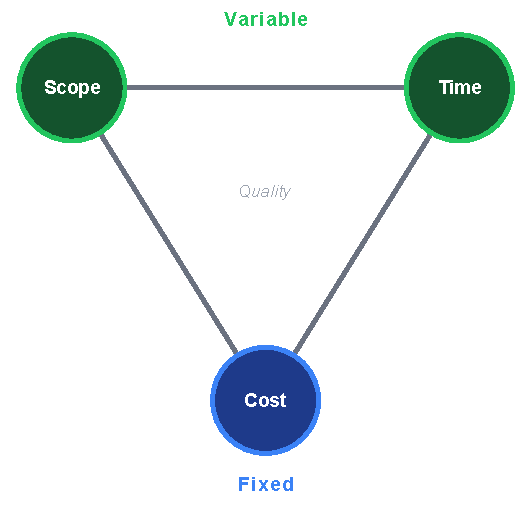
\includegraphics[width=0.40\linewidth]{perm6_VVF.pdf}
\caption{Scope Variable, Time Variable, Cost Fixed.}
\end{figure}

\begin{center}
\begin{tabular}{ccc}
\toprule
Scope & Time & Cost \\
\midrule
\textbf{V} & \textbf{V} & F \\
\bottomrule
\end{tabular}
\end{center}

\noindent\textbf{What it means:} The budget is the only non-negotiable.
Scope and schedule are negotiated continuously within that envelope.

\noindent\textbf{When to use it:} Startups with a fixed runway,
exploratory research and development where the deliverable is unknown a
priori, charitable projects with a fixed grant, or any situation where
the funding envelope is the hard constraint and the team continuously
re-prioritises what to build and when.

\noindent\textbf{Pivot signal:} The budget ceiling is being approached
without a shippable product $\to$ scope must be cut dramatically or a
new funding round (pivot of the cost constraint itself) must be pursued.

\section{Why All-Fixed or All-Variable Does Not Work}
\label{sec:degenerate}

\subsection{All Fixed (F $\cdot$ F $\cdot$ F)}

\begin{figure}[H]
\centering
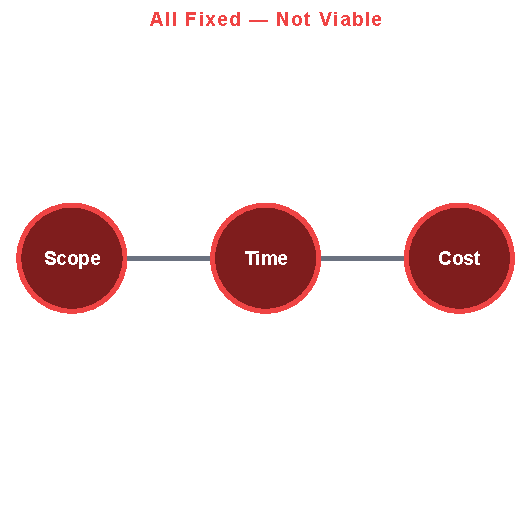
\includegraphics[width=0.40\linewidth]{degen_FFF.pdf}
\caption{All Fixed --- not viable.}
\end{figure}

\begin{center}
\begin{tabular}{ccc}
\toprule
Scope & Time & Cost \\
\midrule
F & F & F \\
\bottomrule
\end{tabular}
\end{center}

\noindent
Fixing all three constraints simultaneously assumes the project can be
planned with perfect precision and that no change will ever occur. In
practice this is impossible because:

\begin{itemize}[leftmargin=*]
  \item \textbf{Reality changes.} Requirements evolve, dependencies
  shift, risks materialise.
  \item \textbf{Estimation is imprecise.} All three estimates carry
  uncertainty; fixing all three means there is no slack to absorb any of
  that uncertainty.
  \item \textbf{The system becomes brittle.} When the first deviation
  occurs (and it always does), there is no sanctioned variable to absorb
  it. The team is forced into covert trade-offs --- hidden overtime,
  silent quality reduction, undisclosed scope cuts --- none of which are
  visible to stakeholders.
  \item \textbf{It creates a culture of false reporting.} Because no
  legitimate flex exists, teams learn to report green status until the
  project collapses.
\end{itemize}

\begin{quote}
All-fixed is not a plan; it is a wish with no contingency.
\end{quote}

\subsection{All Variable (V $\cdot$ V $\cdot$ V)}

\begin{figure}[H]
\centering
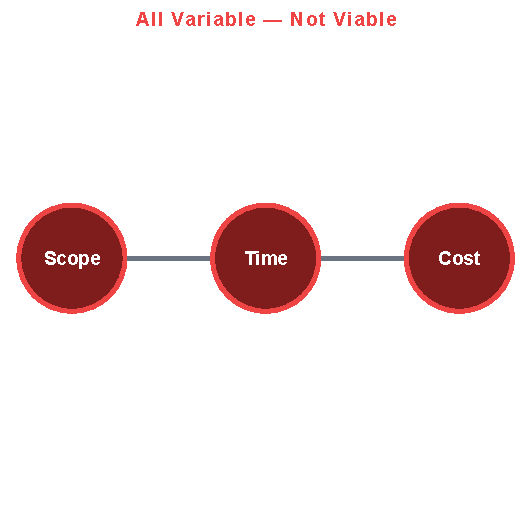
\includegraphics[width=0.40\linewidth]{degen_VVV.pdf}
\caption{All Variable --- not viable.}
\end{figure}

\begin{center}
\begin{tabular}{ccc}
\toprule
Scope & Time & Cost \\
\midrule
\textbf{V} & \textbf{V} & \textbf{V} \\
\bottomrule
\end{tabular}
\end{center}

\noindent
Making all three constraints variable simultaneously removes all
meaningful accountability and direction:

\begin{itemize}[leftmargin=*]
  \item \textbf{There is no target to optimise toward.} Without at least
  one fixed point, there is no way to define success or failure.
  \item \textbf{Scope, schedule, and budget all drift indefinitely.}
  Each individual change feels justified, but the cumulative effect is a
  project that never ends and never delivers.
  \item \textbf{Stakeholder alignment collapses.} Different stakeholders
  implicitly assume different constraints are fixed; with none formally
  anchored, every review meeting reopens every decision.
  \item \textbf{It is not agility --- it is chaos.} Agile methods work
  precisely because they \emph{do} fix at least one dimension (the
  time-box or the team size/cost), making the model a 6-configuration
  problem, not an unconstrained one.
\end{itemize}

\begin{quote}
All-variable is not flexibility; it is the absence of a project.
\end{quote}

\section{Summary Table}
\label{sec:summary}

\begin{center}
\begin{tabular}{c c c c l}
\toprule
\# & Scope & Time & Cost & Methodology / Pattern \\
\midrule
1 & F           & F           & V           & Regulatory / Hard-Deadline Compliance \\
2 & F           & V           & F           & Internal Migration / Capped-Budget Delivery \\
3 & V           & F           & F           & Scrum / Agile Sprint \\
4 & F           & V           & V           & Cost-Plus Contract \\
5 & V           & F           & V           & Ship-to-Date / Market Launch \\
6 & V           & V           & F           & Lean Startup / Fixed Runway / Exploratory R\&D \\
\midrule
--- & F & F & F & {\color{red!70!black}Not viable} (all fixed) \\
--- & V & V & V & {\color{red!70!black}Not viable} (all variable) \\
\bottomrule
\end{tabular}
\end{center}

\medskip
\noindent\textbf{F} = Fixed (blue in diagrams) $\cdot$ \textbf{V} =
Variable (green in diagrams) $\cdot$ interior label \emph{Quality} =
the outcome dimension implicitly governed by the chosen configuration.

\begin{thebibliography}{99}

\bibitem{atkinson1999}
Atkinson, R. (1999). Cost, time and quality, two best guesses and a
phenomenon, its time to accept other success criteria. \emph{Information
Systems Journal}, 9(3), 337--342.

\bibitem{barnes1969}
Barnes, M. (1969). \emph{Time, cost and quality --- the three constraints
of project management}. Proceedings of the Symposium on the Control of
Engineering Design. Institution of Mechanical Engineers.

\bibitem{beck1999}
Beck, K. (1999). \emph{Extreme Programming Explained: Embrace Change}.
Addison-Wesley.

\bibitem{goldratt1997}
Goldratt, E. M. (1997). \emph{Critical Chain}. North River Press.

\bibitem{kerzner2017}
Kerzner, H. (2017). \emph{Project Management: A Systems Approach to
Planning, Scheduling, and Controlling} (12th ed.). Wiley.

\bibitem{poppendieck2003}
Poppendieck, M., \& Poppendieck, T. (2003). \emph{Lean Software
Development: An Agile Toolkit}. Addison-Wesley.

\bibitem{pmi2017}
Project Management Institute. (2017). \emph{A Guide to the Project
Management Body of Knowledge (PMBOK\textsuperscript{\textregistered}
Guide)} (6th ed.). PMI.

\bibitem{ries2011}
Ries, E. (2011). \emph{The Lean Startup: How Today's Entrepreneurs Use
Continuous Innovation to Create Radically Successful Businesses}. Crown
Business.

\bibitem{stapleton2003}
Stapleton, J. (2003). \emph{DSDM: Business Focused Development} (2nd
ed.). Addison-Wesley.

\bibitem{sutherland2020}
Sutherland, J., \& Schwaber, K. (2020). \emph{The Scrum Guide}.
Scrum.org. \url{https://scrumguides.org}

\bibitem{wysocki2014}
Wysocki, R. K. (2014). \emph{Effective Project Management: Traditional,
Agile, Extreme} (7th ed.). Wiley.

\end{thebibliography}

\end{document}
